\documentclass{parcfd2018}

\usepackage{graphicx}
\usepackage{amsmath}
\usepackage{amsfonts}
\usepackage{amssymb}

\title{THREE-DIMENSIONAL FLOW SIMULATIONS OF THE FLYING SNAKE USING MICROSOFT AZURE}

\author{OLIVIER MESNARD$^{*}$ AND LORENA A. BARBA$^{*}$}

\heading{Olivier Mesnard and Lorena A. Barba}

\address{$^{*}$ Department of Mechanical and Aerospace Engineering\\
The George Washington University\\
800 22nd St NW, Washington, DC 20052, United-States\\
e-mail: maeng@gwu.edu, web page: https://www.mae.seas.gwu.edu}

\keywords{Microsoft Azure, Flying snake, PETSc, AmgX}

\abstract{We use our PETSc-based immersed-boundary method code PetIBM to perform three-dimensional flow simulations of the flying snake on the public cloud platform Microsoft Azure.
The simulations ran on NC24r instances using Azure Batch service and Batch Shipyard, solving the Poisson system on multiple GPU devices with Nvidia AmgX library.}

\begin{document}
%\maketitle

We have developed PetIBM\footnote{PetIBM: https://github.com/barbagroup/PetIBM}, a PETSc-based open-source code that solves the Navier-Stokes equations with a fully discrete projection method and various immersed-boundary techniques.
In the present work, we use a decoupled immersed-boundary projection method\cite{Li_et_al_2016} that requires to solve iteratively a Poisson system every time step.
To accelerate the time to solution, we use Nvidia AmgX library\footnote{Nvidia AmgX: https://github.com/NVIDIA/AMGX} to solve the Poisson system on multiple CUDA-capable GPU devices.
The interface between PETSc and AmgX is handled with our in-house wrapper, AmgXWrapper\cite{AmgXWrapper}.\\

Using PetIBM, we investigate the aerodynamics of the \textit{Chrysopelea paradisi}, a species of arboreal snake capable to jump and glide in the air.
Previous experimental work \cite{Holden_et_al_2014} and two-dimensional simulations\cite{Krishnan_et_al_2014, Mesnard_Barba_2017} have reported lift-force enhancement when the glider forms a $35$-degree angle of attack.
We now study the flow around a three-dimensional model, a cylinder with an anatomically accurate cross-section of the gliding snake, at Reynolds number $2000$ and for the particular $35$-degree angle of attack on a structured Cartesian mesh with $233$ million cells.\\

Thanks to a Microsoft Azure sponsorship, we use the cloud platform to run container-based multi-instance tasks for our PetIBM application of the flying snake on NC24r instances (featuring Nvidia K80 GPU devices) with Azure Linux virtual machines and over the Infiniband/RDMA network.
We created the compute pool with Azure Batch, a platform service for running HPC applications in the cloud that relieves the user from manually managing a cluster and tasks scheduling.
Finally, we used Batch Shipyard\footnote{Batch Shipyard: https://github.com/Azure/batch-shipyard}, an open-source software, to provision and execute container-based tasks on Azure Batch nodes.
We see Microsoft Azure as a suitable alternative to traditional University HPC clusters to rapidly develop CFD applications in a cost-efficient manner.

\begin{figure}[!h]
\centering
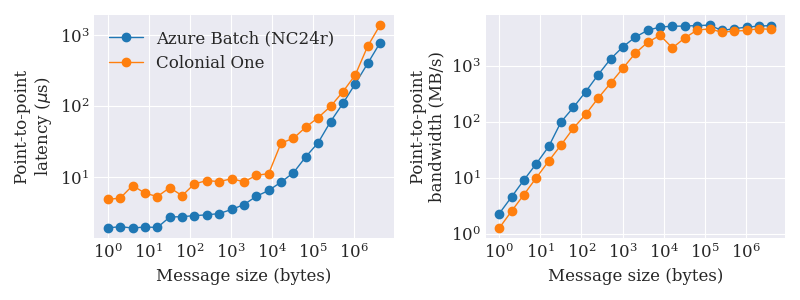
\includegraphics[width=14cm]{figures/latencyBandwidthColonialOneAzure.png}
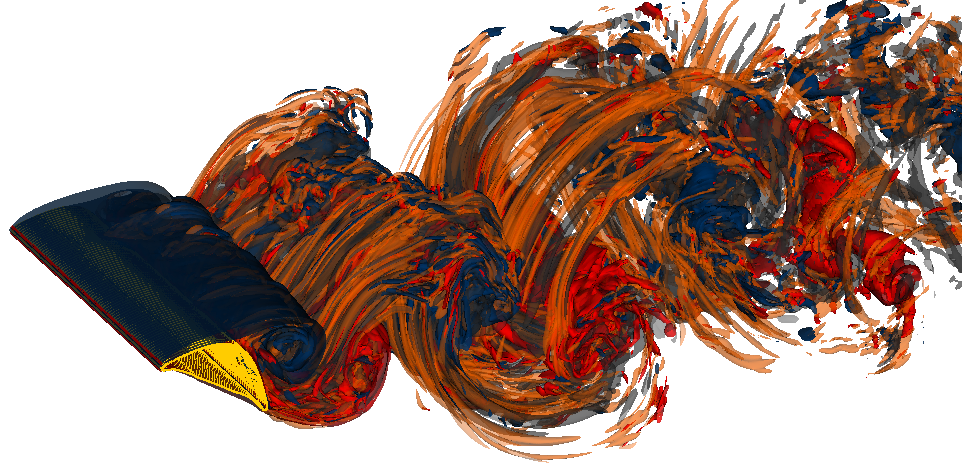
\includegraphics[width=11cm]{figures/wz_wx_wake3d_2k35_meshB_0026.png}
\caption{Top: Point-to-point latency (left) and bandwidth (right) tests performed on a compute pool of two NC24r Azure instances compared with results obtained on our University HPC cluster Colonial One.
Bottom: Streamwise and spanwise vorticity contours after 141.2 time units of flow simulation for the snake cylinder at Reynolds number $2000$ and angle of attack $35^o$ on a 233-million cells grid.}
\label{latency_bandwidth_wz_wx}
\end{figure}

\footnotesize
\begin{thebibliography}{99}
\bibitem{Li_et_al_2016}  Li, R.Y., Xie, C.M., Huang, W.X., and Xu, C.X. (2016). \textit{An efficient immersed boundary projection method for flow over complex/moving boundaries}. Computers \& Fluids, 140, 122-135.
\bibitem{AmgXWrapper}  Chuang, P. and Barba, L.A. (2017). \textit{AmgXWrapper: An interface between PETSc and the NVIDIA AmgX library}. Journal of Open Source Software, 2(16), 280, doi:10.21105/joss.00280.
\bibitem{Holden_et_al_2014}  Holden, D., Socha, J.J., Cardwell, N.D., and Vlachos, P.P. (2014). \textit{Aerodynamics of the flying snake Chrysopelea paradisi: how a bluff body cross-sectional shape contributes to gliding performance}. Journal of Experimental Biology, 217(3), 382-394.
\bibitem{Krishnan_et_al_2014} Krishnan, A., Socha, J.J., Vlachos, P.P., and Barba, L.A. (2014). \textit{Lift and wakes of flying snakes}. Physics of Fluids, 26(3), 031901.
\bibitem{Mesnard_Barba_2017}  Mesnard, O. and Barba, L.A. (2017). \textit{Reproducible and Replicable Computational Fluid Dynamics: It's Harder Than You Think}. Computing in Science \& Engineering, 19(4), 44-55.
\end{thebibliography}

\end{document}
